% Figure from MATH 591 notes, section 67. Added, not from lecture (Lecture 24): the three kinds of maximal integral curve.
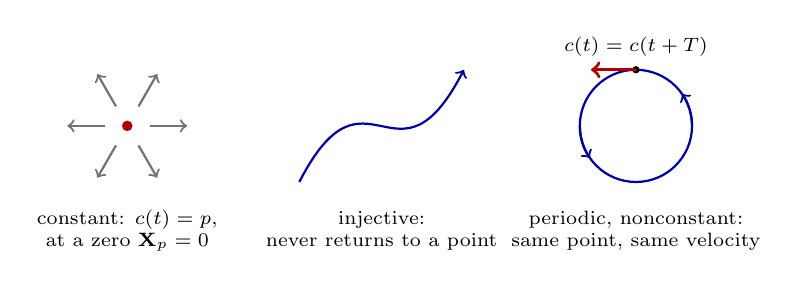
\begin{tikzpicture}[scale=0.95]
\foreach \a in {0,60,...,300} { \draw[->, black!55, thick] ({0.3*cos(\a)},{0.3*sin(\a)}) -- ({0.8*cos(\a)},{0.8*sin(\a)}); }
\fill[red!70!black] (0,0) circle (2pt);
\node[font=\scriptsize, align=center] at (0,-1.4) {constant: $c(t) = p$,\\ at a zero $\mathbf{X}_p = 0$};
\begin{scope}[xshift=3.4cm]
\draw[thick, blue!70!black, ->] (-1.1,-0.75) .. controls (-0.2,1.0) and (0.2,-1.0) .. (1.1,0.75);
\node[font=\scriptsize, align=center] at (0,-1.4) {injective:\\ never returns to a point};
\end{scope}
\begin{scope}[xshift=6.8cm]
\draw[thick, blue!70!black] (0,0) circle (0.75);
\draw[->, thick, blue!70!black] (0.75,0) arc (0:35:0.75);
\draw[->, thick, blue!70!black] (-0.75,0) arc (180:215:0.75);
\fill (0,0.75) circle (1.4pt);
\draw[->, very thick, red!70!black] (0,0.75) -- (-0.6,0.75);
\node[font=\scriptsize, above] at (0,0.8) {$c(t) = c(t + T)$};
\node[font=\scriptsize, align=center] at (0,-1.4) {periodic, nonconstant:\\ same point, same velocity};
\end{scope}
\end{tikzpicture}
